\section{Auswertung}
\subsection{Längenmessung}
Es werden die Längen von vier verschiedenen Koaxialkabeln bestimmt.
Dazu wird der zeitliche Abstand zwischen einlaufendem und 
reflektierten Signal auf einem Oszilloskop betrachtet.\\
In den Abbildungenn~\ref{fig:laenge_rot},~\ref{fig:laenge_schwarz},
~\ref{fig:laenge_gruen} und ~\ref{fig:laenge_trommel} sind die 
verwendeten Bilder zu sehen. Die Zeitmessung wird an den dort 
rot eingezeichneten Markierungen vorgenommen.\\
In Tabelle~\ref{tab:laengenmessung} sind die abgelesenen Zeitabstände 
eingetragen. Ebenso in dieser Tabelle sind die mit den Zeitabständen 
mit Hilfe von Formel~\eqref{eq:laengenrechnung} errechneten 
Längen der Kabel eingetragen. Dabei bezeichnet c die Lichtgeschwindigkeit. 
Der Wert \SI{2.25}{} gibt den Dielektrizitätswert der Kabel an.
%
\begin{equation}
L = \frac{c\cdot\Delta t}{2\cdot\sqrt{2,25}}
\label{eq:laengenrechnung}
\end{equation}
%
\begin{table}[h]
  \centering
  \begin{tabular}{SS|S}
    \toprule
{Kabel}&{Signalabstand }$\Delta${t/}\si{\nano\second}&{Kabellänge/}\si{\metre}\\
\midrule
{Rot}&18&1.8\\
{Schwarz}&116&11.6\\
{Grün}&85&8.5\\
{Trommel}&822&82.1\\
\bottomrule
  \end{tabular}
  \caption{LÄNGENMSSSUNG.}
  \label{tab:laengenmessung}
\end{table}
%
\begin{figure}[]
\centering
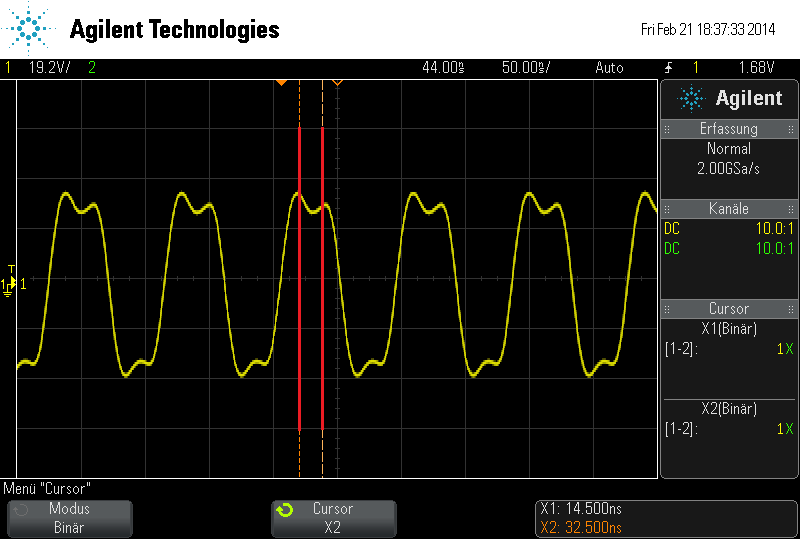
\includegraphics[width=0.8\textwidth]{laenge_rot.png}
\caption{ROT}
\label{fig:laenge_rot}
\end{figure}
%
\begin{figure}[]
\centering
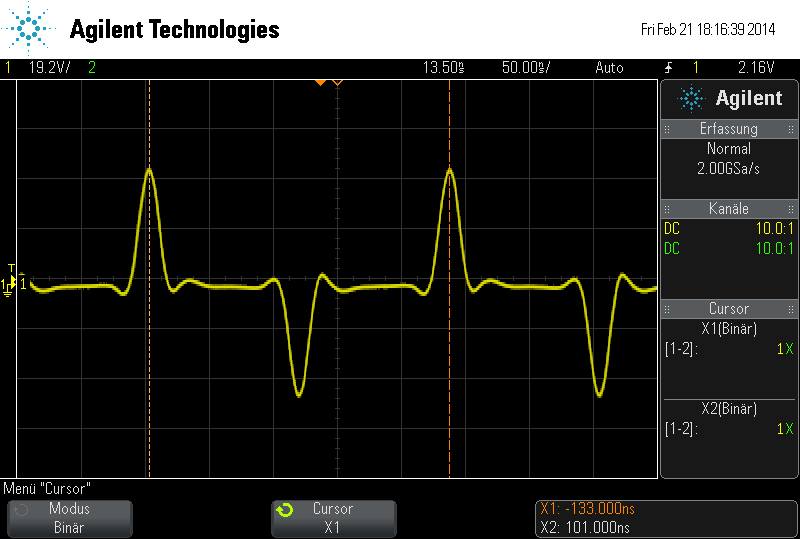
\includegraphics[width=0.8\textwidth]{laenge_schwarz.png}
\caption{SCHWARZ}
\label{fig:laenge_schwarz}
\end{figure}
%
\begin{figure}[]
\centering
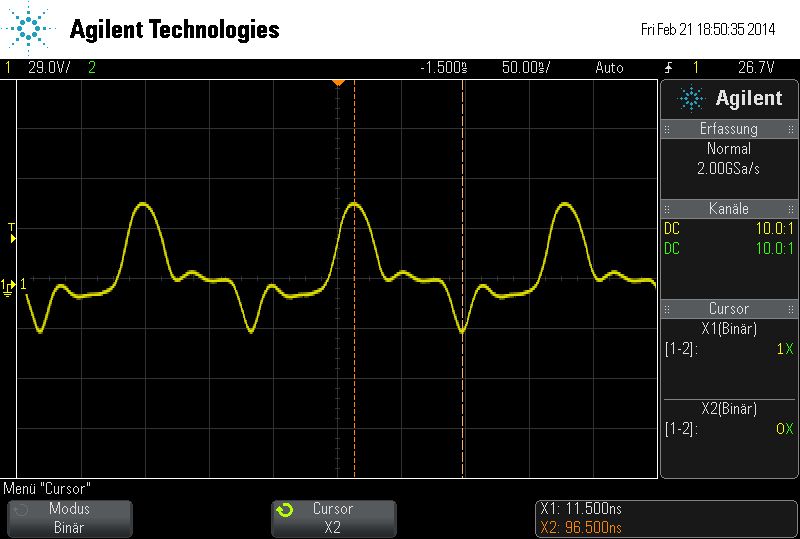
\includegraphics[width=0.8\textwidth]{laenge_gruen.png}
\caption{GRÜN}
\label{fig:laenge_gruen}
\end{figure}
%
\begin{figure}[]
\centering
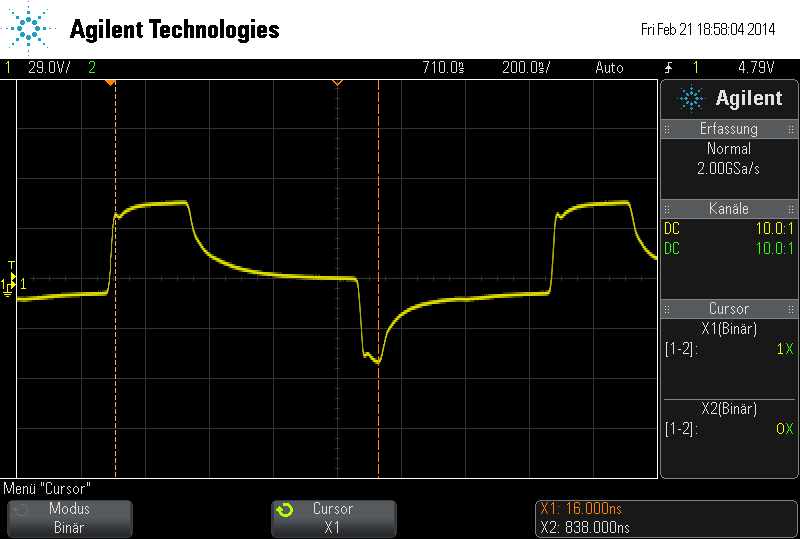
\includegraphics[width=0.8\textwidth]{laenge_trommel.png}
\caption{TROMMEL}
\label{fig:laenge_trommel}
\end{figure}
%
\FloatBarrier
%
\subsection{Belagsmessung}
%
Die mit einem LRC-Messgerät bestimmten Induktivitäten ${L}_{g}$, 
Widerstände ${R}_{g}$ und Kapazitäten ${C}_{g}$ bei verschiedenen 
Frequenzen f sind für das rote Kabel in 
Tabelle~\ref{tab:RLC_rot}, für das schwarze Kabel in 
Tabelle~\ref{tab:RLC_schwarz}, und für die Kabeltrommel in 
Tabelle~\ref{tab:RLC_trommel} aufgeführt.
Ebenfalls in diesen Tabellen sind sowohl die mit
Formel~\eqref{eq:G-FORMEL} berechneten Querleitwerte ${G}_{g}$ 
der jeweiligen Kabel aufgeführt, als auch die durch die Längen der 
Kabel errechneten Beläge R, L, C und G.
%
\begin{table}[h]
  \centering
  \begin{tabular}{SSSSSSSSS}
    \toprule
{f /}\si{\kilo\hertz}&
${R}_{g}${/}\si{\ohm}&{R/}\si{\ohm\per\metre}&
${L}_{g}${/}\si{\micro\henry}&{L/}\si{\micro\henry\per\metre}&
${C}_{g}${/}\si{\pico\farad}&{C/}\si{\pico\farad\per\metre}&
${G}_{g}${/}\si{\micro\siemens}&{G/}\si{\micro\siemens\per\metre}\\
\midrule
0.05&2.47&1.37&4.5&2.50&138.8&77.2&76.2&42.4\\
0.10&2.48&1.38&4.5&2.50&138.8&77.2&76.5&42.5\\
0.20&2.48&1.38&4.4&2.45&138.8&77.2&78.2&43.5\\
0.30&2.48&1.38&4.6&2.56&138.8&77.2&74.8&41.6\\
0.50&2.48&1.38&4.5&2.50&138.8&77.2&76.5&42.5\\
0.80&2.48&1.38&4.3&2.40&138.8&77.2&80.0&44.5\\
1.00&2.49&1.38&4.2&2.33&138.8&77.2&82.3&45.7\\
1.50&2.49&1.38&4.1&2.28&138.8&77.2&84.3&46.9\\
2.00&2.50&1.39&4.0&2.22&138.7&77.1&86.7&48.2\\
3.00&2.51&1.40&3.8&2.10&138.7&77.1&92.3&51.3\\
5.00&2.53&1.41&3.4&1.89&138.6&77.1&103.1&57.3\\
7.00&2.55&1.42&3.2&1.78&138.6&77.1&110.4&61.4\\
10.00&2.56&1.42&3.0&1.67&138.6&77.1&118.3&65.8\\
14.00&2.58&1.43&2.8&1.56&138.5&77.0&127.6&70.9\\
18.00&2.59&1.44&2.8&1.56&138.5&77.0&128.1&71.2\\
20.00&2.60&1.45&2.7&1.50&138.5&77.0&133.4&74.1\\
100.00&2.60&1.45&2.6&1.45&138.6&77.1&138.6&77.1\\
\bottomrule
  \end{tabular}
  \caption{RLCROT}
  \label{tab:RLC_rot}
\end{table}
%
\begin{table}[h]
  \centering
  \begin{tabular}{SSSSSSSSS}
    \toprule
{f /}\si{\kilo\hertz}&
${R}_{g}${/}\si{\ohm}&{R/}\si{\ohm\per\metre}&
${L}_{g}${/}\si{\micro\henry}&{L/}\si{\micro\henry\per\metre}&
${C}_{g}${/}\si{\pico\farad}&{C/}\si{\pico\farad\per\metre}&
${G}_{g}${/}\si{\micro\siemens}&{G/}\si{\micro\siemens\per\metre}\\
\midrule
0.05&2.47&1.37&4.5&2.50&138.8&77.2&76.2&42.4\\
\bottomrule
  \end{tabular}
  \caption{RLCSCHWARZ}
  \label{tab:RLC_schwarz}
\end{table}
%
\begin{table}[h]
  \centering
  \begin{tabular}{SSSSSSSSS}
    \toprule
{f /}\si{\kilo\hertz}&
${R}_{g}${/}\si{\ohm}&{R/}\si{\ohm\per\metre}&
${L}_{g}${/}\si{\micro\henry}&{L/}\si{\micro\henry\per\metre}&
${C}_{g}${/}\si{\pico\farad}&{C/}\si{\pico\farad\per\metre}&
${G}_{g}${/}\si{\micro\siemens}&{G/}\si{\micro\siemens\per\metre}\\
\midrule
0.05&2.47&1.37&4.5&2.50&138.8&77.2&76.2&42.4\\
\bottomrule
  \end{tabular}
  \caption{RLCTROMMEL}
  \label{tab:RLC_trommel}
\end{table}
%
Einen Plot der Leitungsbelagswerte in Abhängigkeit von der Frequenz 
für die verschiedenen Kabel ist in Plot~\ref{fig:belaege} zu sehen.
%
HIER 4ER PLOT REIN
%
\subsection{Dämpfungsbestimmung}
%
Um die Dämpfungskonstante $\alpha$ der Kabeltrommen zu bestimmen, 
wird die Fouriertransformation eines Rechtecksignals betrachtet. Die 
für ein sehr kurzes Kabel und die Kabeltrommen erhaltenen FFT-Bilder 
sind in den Bildern~\ref{fig:daempfung_kurz} 
und~\ref{fig:daempfung_lang} zu sehen.\\
In Tabelle~\ref{tab:daempfung} sind die abgelesenen Amplituden der 
erkennbaren Maxima eingetragen, sowie das Verhältnis von den 
ungedämpften zu den gedämpften Amplituden, welches die 
Dämpfungskonstante $\alpha$ angibt.
%
\begin{figure}[]
\centering
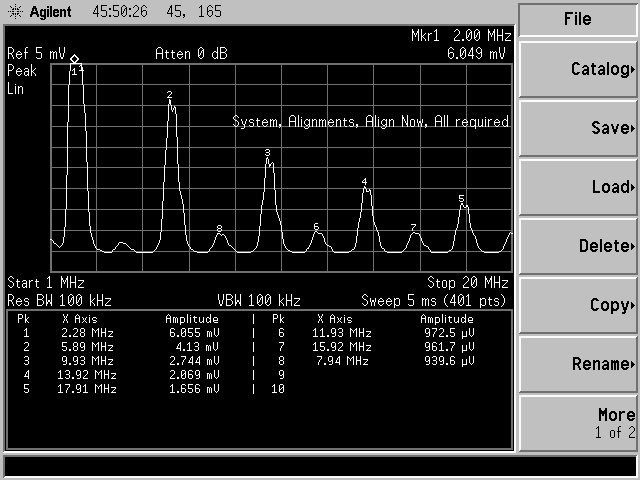
\includegraphics[width=0.8\textwidth]{daempfung_kurz.png}
\caption{KURZ}
\label{fig:daempfung_kurz}
\end{figure}
%
\begin{figure}[]
\centering
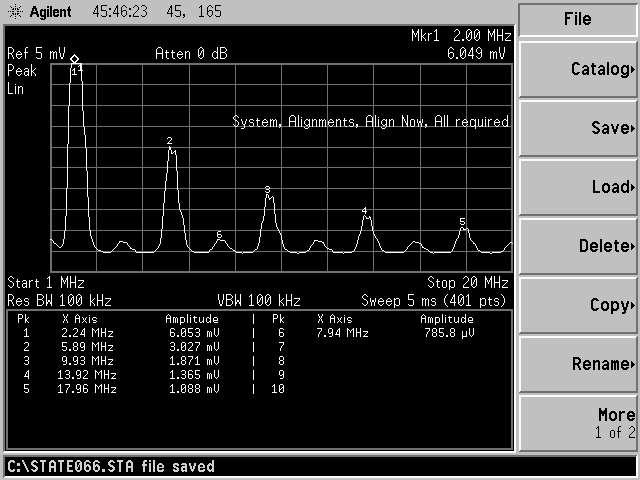
\includegraphics[width=0.8\textwidth]{daempfung_lang.png}
\caption{LANG}
\label{fig:daempfung_lang}
\end{figure}
%
\begin{table}[h]
  \centering
  \begin{tabular}{SSS|S}
    \toprule
{Nr.}&${U}_{ungedämpft}${/}\si{\volt}&${U}_{gedämpft}{ /}\si{\volt}$&
$\frac{{U}_{ungedämpft}}{{U}_{gedämpft}}$\\
\midrule
1&9.8&8.4&1.17\\
2&4.4&3.4&1.30\\
3&3.2&2.4&1.34\\
4&2.6&2.0&1.3\\
5&2.3&1.1&2.10\\
\midrule
\multicolumn{3}{c}{Mittelwert: }&\SI{1.44(15)}{}\\
\bottomrule
  \end{tabular}
  \caption{DÄMPFUNG}
  \label{tab:daempfung}
\end{table}
%
%
\subsection{Mehrfacheflexion}
\subsection{Verschiedene Abschlusswiderstände}